\section{Results}

Firstly, the main results that should answer the research question will be discussed.
After that, a few interesting insights that were gathered after the experiment will be shown.

\subsection{Main Results}
The mean for the static condition is $0.6051$ with a standard deviation of $0.2792$ and the mean for the dynamic condition is $0.8354$ with a standard deviation of $0.0872$.
Shapiro-Wilk test for both the static and dynamic data is not significant ($p = 0.0776$ and $p = 0.0592$ respectively), which means that an independent sample t-test can be performed. %when I have 6000 samples this becomes 0.1818 and 0.1192
The indepedent sample t-test showed that the data is significantly different ($p = 0.00006335$).
This means that the hypothesis that sexual reproduction is more advantageous than asexual reproduction in a faster changing environment can be accepted under this experiment.

\subsection{Descriptives}
To get a good insight in the data, it is interesting to see what happens over iterations, since properties such as average crossover, average fitness and age of food will change over time.
Figure \ref{fig:avgcross} shows the average crossover of the two different conditions over time.
The results that are shown are averaged over all $30$ runs.
The average crossover for the static condition declines slowly, but steadily over time.
It shows that although it has a high average of crossover, it keeps declining.
The average of crossover in the dynamic condition is quite steady, and apart from small fluctutations does not change.
Figure \ref{fig:avgfit} shows the average fitness (age of the agents) of the two different conditions over time.
It shows that in the static condition the average fitness increases to a high amount (up to $5,000$) and that it is very low in the dynamic condition (fluctuating around $200$).
Figure \ref{fig:avgfood} shows the average age of the food in both conditions.
The age of the food in the dynamic condition is the most prominent, since in the beginning it is relatively high and decreases over time (albeit with heavy fluctuations).
The age in the static condition stays very steady.
Figure \ref{fig:avgpois} shows the average age of the poison in both conditions.
In the static condition, the age increases by a large amount, whereas in the dynamic condition the age of the poison stays relatively low.
In the dynamic condition, the age of the food and the poison stay quite the same (around the $2,500$ lowering down to $1,000$).

\begin{figure}[H]
\centering
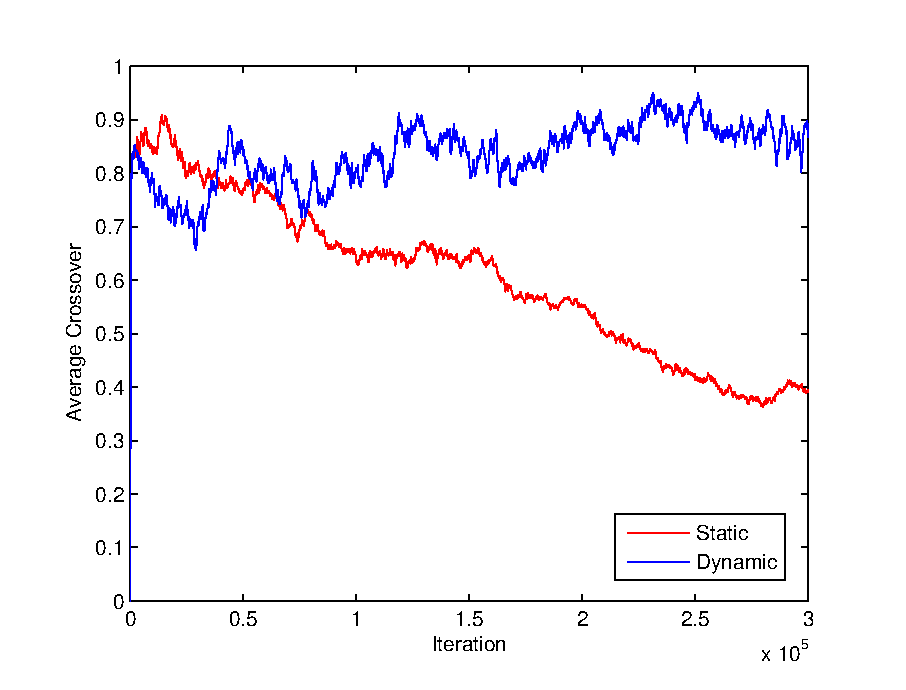
\includegraphics[width=0.75\textwidth]{average_crossover.eps}
\caption{Average crossover per condition. The results shown here are averaged over all $30$ runs.}
\label{fig:avgcross}
\end{figure}

\begin{figure}[H]
\centering
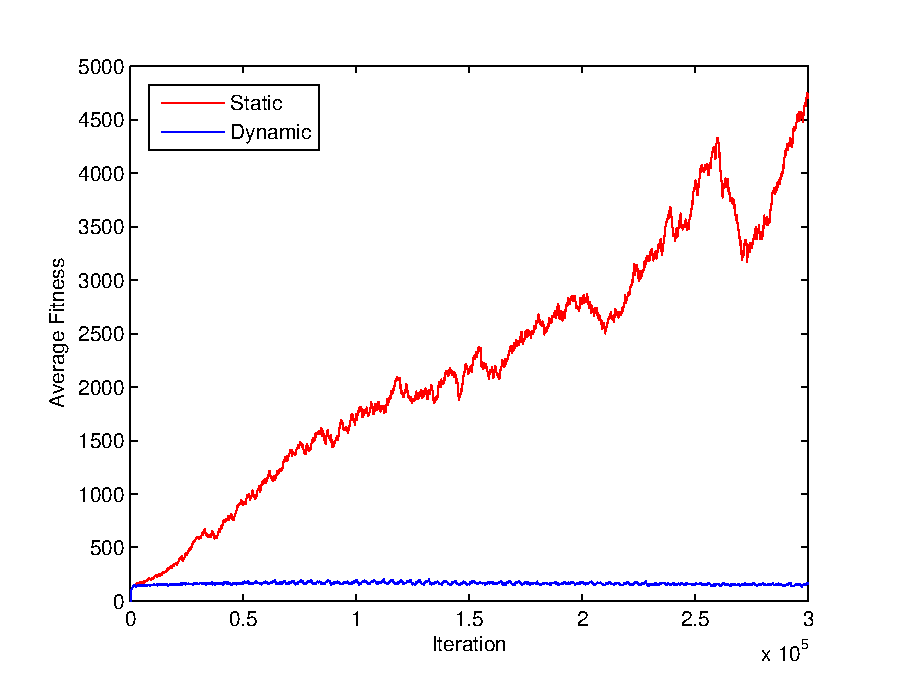
\includegraphics[width=0.75\textwidth]{average_fitness.eps}
\caption{Average fitness per condition. The results shown here are averaged over all $30$ runs.}
\label{fig:avgfit}
\end{figure}

\begin{figure}[H]
\centering
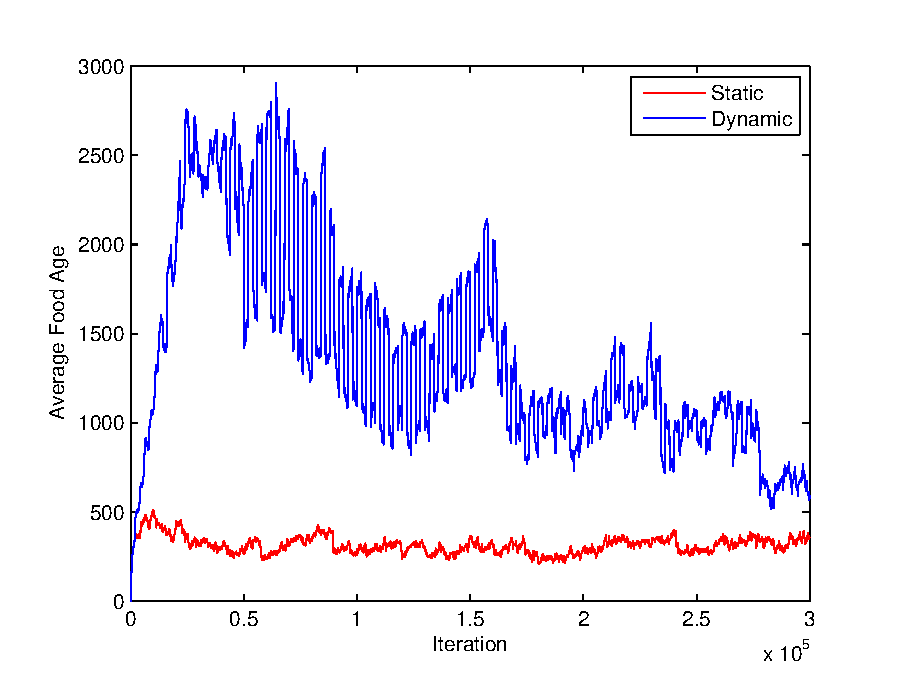
\includegraphics[width=0.75\textwidth]{average_food_age.eps}
\caption{Average age of food per condition. The results shown here are averaged over all $30$ runs.}
\label{fig:avgfood}
\end{figure}

\begin{figure}[H]
\centering
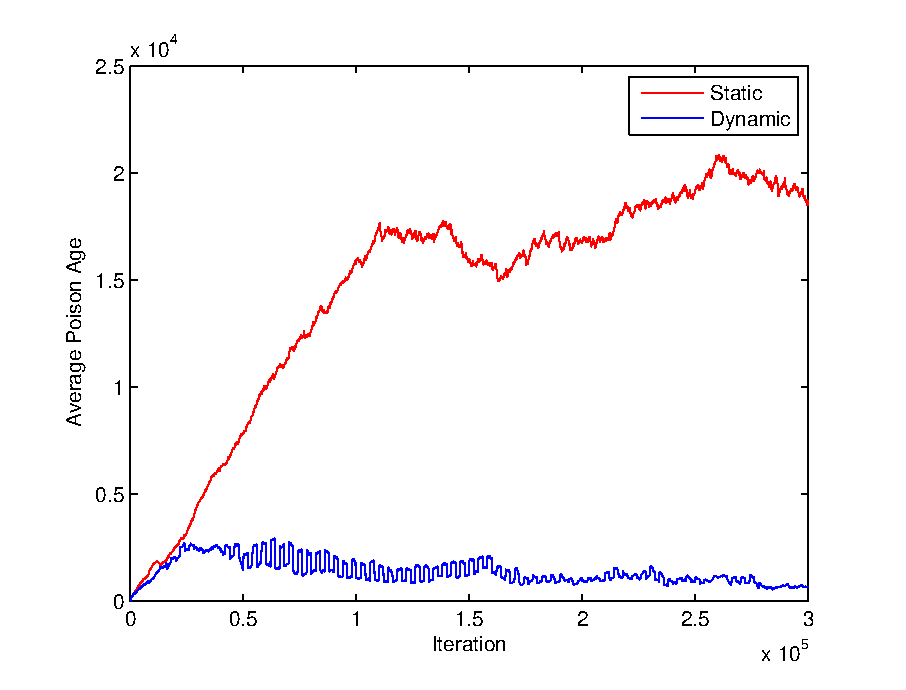
\includegraphics[width=0.75\textwidth]{average_poison_age.eps}
\caption{Average age of poison per condition. The results shown here are averaged over all $30$ runs.}
\label{fig:avgpois}
\end{figure}